% ---------------------------------------------------
% ----- Chapters of the template
% ----- for Bachelor-, Master thesis and class papers
% ---------------------------------------------------
%  Created by C. Müller-Birn on 2012-08-17, CC-BY-SA 3.0.
%  Freie Universität Berlin, Institute of Computer Science, Human Centered Computing. 
%
\chapter{Evaluationen}
\label{chap:evaluation}
		
		Im Rahmen dieser Masterarbeit wurden mehrere Evaluationen durchgeführt, um die
		Genauigkeit der Matcher zu beurteilen. In diesem Prozess wurde etablierte
		Matching Software für ausgewählte Ontologien verwendet, um eine möglichst
		umfangreiche Ergebnismenge für den Vergleich zu haben.
		
		\section{Evaluation 1}
		\label{subsec:Evaluation 1}
		Als erste Evaluation wurde ein Vergleich zwischen einem von Dr. Ing. Alsayed
		Algergawy entwickelten Algorithmus und einem Matching Prozess mit den Simple
		Label und Levenshtein Distance Matchern. Anschließend wurden die Ergebnisse
		händisch begutachtet, um die Qualität der Matchings zu beurteilen. Die
		Algorithmen nehmen als Ausgangsbasis beide die Labels der Elemente der
		Ontologien.
		
		\subsection{Verwendete Ontologien}
		Für den Vergleich wurden die Environment Ontology (EnvO) und die Phenotypic
		Quality Ontology (PATO) herangezogen. EnvO wurde entwickelt, um die
		Annotation für jegliche Organismen und biologische Exemplare zu erleichtern.
		Dafür wird ein strukturiertes Vokabular geboten. EnvO besteht aus Wörtern für
		Biome, Umwelteigenschaften und
		Materialien.\footnote{\url{http://www.environmentontology.org/home/about-envo}}
		PATO enthält Begriffe über
		Phänotypen, also das
		Erscheinungsbild von
		Organismen.\footnote{\url{http://obofoundry.org/ontology/pato.html}}
		
		\subsection{Resultat}
		Insgesamt wurden 203 Matchings von beiden Algorithmen gefunden, bis auf neun
		Ergebnisse beschrieben alle das gleiche, d.h. sie hatten die selbe URI.
		Wenn man die exklusiven Ergebnisse betrachtet, also solche, die nur einer
		der beiden Matching Algorithmen gefunden hat, dann hat der Simple Ontology
		Matcher fand 89 potenzielle Matchings, während der Algorithmus von Dr. Ing.
		Algergawy 62 vorschlug. Von diesen Matchings war beim Simple Ontology Matcher
		lediglich eines dabei, bei welchem beide Elemente die gleiche URI hatten. Bei
		den Ergebnissen anderen Algorithmus war dies bei 19 Matchings der Fall.\\
		Alle Paare und die konkrete Einteilung in die Kategorien sind im Appendix
		\ref{app:first_appendix}
		aufgeführt.
		
		\subsection{Korrektheit der Resultate}
		Die erste Evaluation sollte als erste grobe Einordnung dienen, inwiefern
		der Simple Ontology Matcher seinem Ziel nahe kommt, zwei beliebige Ontologien
		zu vergleichen und Verbindungen zwischen ihnen zu finden. Für die Einordnung
		wurden folgende Kategorien verwendet:\\
		\begin{itemize}
		  \item Gleich: Zwei Elemente beschreiben das selbe Konzept
		  \item Gegenteil: Zwei Elemente sind das Gegenteil voneinander
		  \item Indirekt: Die beiden Elemente können über ein anderes Elemente
		  miteinander verbunden werden, unabhängig davon, ob es Teil einer der beiden
		  Ontologien ist
		  \item Ähnlich: Zwei Elemente sind zwar verbunden, es lässt sich aber keine
		  direkte Verbindung angeben, meist ist eines eine Beschreibung des anderen
		  oder beide haben den selbst Wortstamm
		  \item Keine: Es besteht keine Verbindung und das Matching ist ein false
		  positive
		  \item Unsicher: Es ist unklar ob zwei Elemente miteinander verbunden sind,
		  da das notwendige Domänenwissen aufgrund von Fachfremdheit fehlt.
		\end{itemize}
		
		Bei der Durchsicht der Ergebnisse fiel schnell auf, dass der Simple Ontology
		Matcher sehr viele Matchings gefunden hat, die zwar verbunden sind, aber keine
		Gleichheit ausdrücken (Kategorien Gegeteil und indirekt).
		Wohingegen der von Dr. Ing. Algergawy verwendete Algorithmus viele Matchings
		gefunden hat, die Gleichheit zwischen den Elementen ausdrücken (Kategorien
		Gleich und Ähnlich).\\
		
		\begin{table}[h!]
		\centering
		\small
		\setlength\tabcolsep{2pt}
		\caption{Kategorisierte Ergebnisse}
		\begin{tabular}{|c|c|c|c|c|c|c|}\hline
		Matching Algorithmus von & Gleich & Gegenteil & Indirekt & Ähnlich & Keine &
		Unsicher \\\hline
		Dr. Ing. Algergawy & 6 (13,95\%) & 0 & 1 (2,32\%) & 16 (37,2\%) & 13
		(30,23\%) & 7 (16,27\%) \\\hline
		Schröter & 1 (1,13 \%) & 40 (45,45\%) & 5 (5,68\%) & 11 (12,5\%) & 21
		(23,86\%) & 10 (11,36\%) \\\hline
		\end{tabular}
		\end{table}
		Alle Prozentangaben in der Tabelle wurden abgerundet.\\
				
		\begin{figure}[h!]
		\centering
		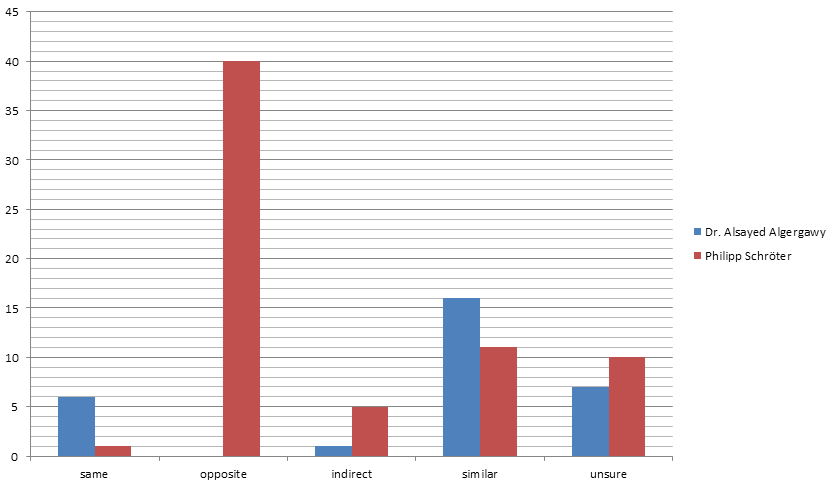
\includegraphics[width=1.0\textwidth]{pics/Vergleich-Algergawy-Schroeter_2016-11-22.png}
		\caption{Vergleich Algergawy Schröter}
		\label{fig16}
		\end{figure}
		
		\subsection{Fazit und Verbesserungen des Simple Ontology Matchers}
		Als erstes wurde für die gleichen Elemente, also solche mit gleicher URI, ein
		eigener Matcher geschrieben und als Bedingung in die anderen Matcher
		aufgenommen, dass die URI nicht mehr gleich sein darf. Dadurch können diese
		trivialen Ergebnisse gezielt in die Ergebnismenge miteinbezogen oder
		ausgeschlossen werden.\\
		Für den Levenshtein Matcher ergibt sich die Verbesserung, dass die obere
		Schranke für mögliche Änderungen nicht nur ein absolutes Maximum benötigt,
		sondern eines, das an die Wortlänge angepasst ist.\\
		Als Gesamterkenntnis hat sich gezeigt, dass es einen Unterschied in der
		Herangehensweise gibt, der zu derartig unterschiedlichen Ergebnissen führt.
		Die übliche Suche nach Verbindungen zwischen Ontologien bezieht sich auf
		Gleichheit oder Ähnlichkeit. Im Rahmen dieser Masterarbeit wurde intuitiv der
		Ansatz gewählt, dass jede möglich Art der Verbindung zu suchen ist, egal
		welcher Art. Ob und wo diese Ansätze sinvoll sind, müssen Experten auf dem
		jeweiligen Gebiet entscheiden, auf dem die Matchings erstellt werden.
		
		\section{Evaluation 2}
		\label{subsec:Evaluation 2}
		Anhand eines vorher festgelegten Satzes an Daten wurde der im Rahmen dieser
		Masterarbeit entwickelte Simple Ontology Matcher mit der etablierten Matching
		Software
		AgreementMakerLight\footnote{\url{https://github.com/AgreementMakerLight/AML-Jar}}(\textit{AML})
		verglichen. Dieser Vergleich dient dazu, die Matcher mittels \textit{Precision
		and recall} zu verbessern.
		
		\subsection{Verwendete Ontologien}
		Für den Vergleich wurden zwei Ontologien verwendet, Human und Mouse. Human
		ist beschreibt die menschliche Anatomie, Mouse die von Mäusen. Diese beiden
		wurden ausgewählt, da eine hohe Überschneidung zu erwarten ist, wobei die
		innerhalb der Ontolgien verwendeten Terminologie ähnlich sein dürfte.
		
		\subsection{Resultat}
		Wenn man die Gesamtheit der Ergebnisse aus beiden Matching Tools betrachtet,
		erhält man eine Gesamtmenge von 2421 potenziellen Matchings. Der Simple
		Ontology Matcher hat 980 Ergebnisse, welche nicht in denen von AML enthalten
		sind (diese werden im Anschluss noch genauer analysiert). AML hat 786
		exklusive Ergebnisse. Der verbliebene Teil von 655 Matchings wurden von beiden
		vorgeschlagen. Die vollständigen Ergebnisse sind in Appendix \ref{app:second_appendix}
		aufgeführt.
		
		\subsection{Korrektheit der Resultate des Simple Ontology Matchers}
		Die exklusiven Ergebnisse des Simple Ontology Matchers wurden händisch auf
		Korrektheit überprüft und in verschiedene Kategorien unterteilt. Die
		Kategorien wurden gegenüber der ersten Evaluation geändert. Die Kategorien
		indirekt und ähnlich wurden entfernt, um nur die konkret zutreffenden
		Ergebnisse einzubeziehen. Die Kategorien sind \textit{gleiches} Element,
		\textit{direkte}, \textit{keine}, \textit{unsichere} Verbindung.\\
		Gleiche Element sind nicht nur Teile der Ontologie, die das
		selbe Konzept darstellen, sondern solche, die die gleiche URI haben, also bei denen
		es sich tatsächlich um ein und dasselbe handelt. Eine direkte Verbindung liegt
		vor, wenn zwischen zwei Elemente eine eindeutige Verknüpfung vorliegt, z.B.
		Unterklasse (rdfs:subClassOf) oder Gegenteil (owl:differentFrom). Wenn
		es unklar ist, ob sich ein korrektes Matching handelt, werden die entsprechenden Paare in die
		Kategorie "`unsicher"' einsortiert. Diese Ergebnisse benötigen zusätzliche
		Betrachtung von Personen mit entsprechendem Hintergrundwissen in der Domäne.\\
		
		\begin{table}[h!]
		\centering
		\caption{Kategorisierte Ergebnisse}
		\begin{tabular}{|c|c|}\hline
		Kategorie & Anzahl Paare\\ \hline
		Gleich & 7\\ \hline
		Direkt & 887\\ \hline
		Keine & 13\\ \hline
		Unsicher & 73\\ \hline
		\end{tabular}
		\end{table}
		
		\subsection{Analyse und mögliche Verbesserung der Matcher}
		Wenn man die vom Simple Ontology Matcher nicht erfassten Ergebnispaare
		betrachtet, fällt als erstes auf, dass es fast ausschließlich Paare mit
		unterschiedlicher Groß- und Kleinschreibung und mit bzw. ohne Unterstriche
		sind.\\
		Beispiele:
		\begin{itemize}
		\item \url{http://mouse.owl#MA_0001849} (right main bronchus) und \url{http://human.owl#NCI_C33486} (Right\textunderscore Main\textunderscore Bronchus)
		\item \url{http://mouse.owl#MA_0000638} (wrist skin) und \url{http://human.owl#NCI_C52752} (Wrist\textunderscore Skin)
		\item \url{http://mouse.owl#MA_0000467} (foot digit 3) und \url{http://human.owl#NCI_C52841} (Foot\textunderscore Digit\textunderscore 3)
		\item \url{http://mouse.owl#MA_0001432} (lumbar vertebra 5) und \url{http://human.owl#NCI_C32903} (L5\textunderscore Vertebra)
		\item \url{http://mouse.owl#MA_0001106} (vagus X nerve) und \url{http://human.owl#NCI_C12812} (Vagus\textunderscore Nerve)
		\item \url{http://mouse.owl#MA_0001426} (cervical vertebra 6) und \url{http://human.owl#NCI_C32244} (C6\textunderscore Vertebra)
		\item \url{http://mouse.owl#MA_0001579} (lip skin) und \url{http://human.owl#NCI_C12291} (Skin\textunderscore of\textunderscore the\textunderscore Lip)
		\item \url{http://mouse.owl#MA_0000370} (kidney capsule) und \url{http://human.owl#NCI_C12885} (Renal\textunderscore Capsule)
		\item \url{http://mouse.owl#MA_0001320} (external naris) und \url{http://human.owl#NCI_C33178} (Nostril)
		\item \url{http://mouse.owl#MA_0000715} (venous system smooth muscle) und \url{http://human.owl#NCI_C49321} (Venous\textunderscore System\textunderscore Smooth\textunderscore Muscle\textunderscore Tissue)
		\item \url{http://mouse.owl#MA_0001735} (epididymal duct) und \url{http://human.owl#NCI_C32484} (Duct\textunderscore of\textunderscore the\textunderscore Epididymis)
		\end{itemize}